\section{Harakatning nisbiyligi}

\begin{enumerate}

\item Avtomobil dvigateli parragi chetki nuqtalarining harakat traektoriyasi:
avtomobil bilan bog‘langan sanoq sistemasiga; yer bilan bog‘langan sanoq sistemasiga nisbatan qanday shaklda bo‘ladi?

\begin{enumerate}[label=\Alph*)]
\item aylana; vintsimon
\item vintsimon; aylana
\item parabola; egri chiziq
\item aylana; aylana
\end{enumerate}


\item Oqimga qarshi suzayotgan bolaning suvga nisbatan tezligi $1.5\ \text{m/s}$,
suvning qirg‘oqqa nisbatan tezligi $0.5\ \text{m/s}$ bo‘lsa,
bolaning qirg‘oqqa nisbatan tezligi qanday (m/s) bo‘ladi?

\begin{enumerate}[label=\Alph*)]
\item 2.5
\item 2
\item 1.5
\item 1

\end{enumerate}


\item Rels ustida $0.4\ \text{m/s}$ tezlik bilan gorizontal harakatlanayotgan kran
yukni $0.3\ \text{m/s}$ tezlik bilan vertikal yuqoriga ko‘tarmoqda.
Yer bilan bog‘langan sanoq tizimida yukning tezligi qanday (m/s)?

\begin{enumerate}[label=\Alph*)]
\item 0.1
\item 0.25
\item 0.35
\item 0.5

\end{enumerate}


\item Suzuvchining suvga nisbatan tezligi $0.9\ \text{m/s}$ ga teng va qirg‘oqqa tik yo‘nalgan,
suvning oqish tezligi esa $1.2\ \text{m/s}$ ga teng.
Suzuvchining qirg‘oqqa nisbatan tezligi qanday (m/s)?

\begin{enumerate}[label=\Alph*)]
\item 0.3
\item 0.9
\item 1.2
\item 1.5

\end{enumerate}


\item Jism harakat tezligining 2 ta tashkil etuvchisi bir-biriga nisbatan
$60^\circ$ burchak ostida yo‘nalgan bo‘lib, modullari mos ravishda
$4$ va $6\ \text{m/s}$ ga teng.
Natijaviy tezlik qanday (m/s)?

\begin{enumerate}[label=\Alph*)]
\item 5
\item 7.7
\item 8.7
\item 10
\item 12.8
\end{enumerate}


\item Metrodagi eskalator odamni yuqoriga $45$ s da olib chiqadi.
Odam va eskalator birgalikda harakat qilsa, odam $15$ s da ko‘tariladi.
Eskalator tinch tursa, odam necha sekundda yuqoriga chiqadi?

\begin{enumerate}[label=\Alph*)]
\item 30
\item 22.5
\item 60
\item 15.5

\end{enumerate}


\item $5\ \text{m/s}$ tezlik bilan esayotgan shamolga qarshi $90\ \text{km/h}$ tezlik bilan harakatlanayotgan avtomobilning
shamolga nisbatan tezligi qanday (m/s)?

\begin{enumerate}[label=\Alph*)]
\item 10
\item 5
\item 30
\item 25

\end{enumerate}


\item Shosseda avtobuslar kolonnasi $30\ \text{km/h}$ tezlik bilan harakatlanmoqda. $70\ \text{km/h}$ tezlik bilan harakatlanayotgan mototsiklchi kolonnani quvib o‘tyapti. Mototsiklning kolonnaga nisbatan tezligi qanday (km/h)?

\begin{enumerate}[label=\Alph*)]
\item 30
\item 40
\item 50
\item 70

\end{enumerate}


\item Asfalt yo‘l bo‘ylab velosipedchi to‘g‘ri chiziqli tekis harakat qilyapti. U yo‘l chetidagi ikki ketma-ket telegraf ustunlari oralig‘idagi masofani $10$ s da bosib o‘tyapti. Ustunlar oralig‘i $50$ m. Velosipedchi qarshisidan kelayotgan avtomobilning spidometri $36$ km/soat ni ko‘rsatyapti. Velosipedchi avtomobilga nisbatan qanday tezlik bilan harakatlanyapti (m/s)?

\begin{enumerate}[label=\Alph*)]
\item 20
\item 25
\item 15
\item 5

\end{enumerate}


\item Ikki avtomobil to‘g‘ri burchak ostida kesishuvchi ikki yo‘l bo‘ylab
harakatlanmoqda. Ulardan biri chorrahaga $16$ m/s tezlik bilan yaqinlashmoqda, ikkinchisi esa $12$ m/s tezlik bilan uzoqlashmoqda. 1-avtomobilning 2-avtomobilga nisbatan tezligi moduli qanday (m/s)?

\begin{enumerate}[label=\Alph*)]
\item 28
\item 20
\item 16
\item 12

\end{enumerate}


\item O‘zaro $60^\circ$ burchak hosil qilib,
yerga nisbatan $v$ tezlik bilan harakatlanayotgan ikki jismning bir-biriga nisbatan tezligining moduli nimaga teng?

\begin{enumerate}[label=\Alph*)]
\item $v/2$
\item $\sqrt{3}v/2$
\item $\sqrt{3}v$
\item $v$

\end{enumerate}


\item Tezliklari $v_1=10$ m/s va $v_2=12$ m/s bo‘lgan jismlar berilgan chizma orqali harakat qilmoqda.
Ularning nisbiy tezligini toping (m/s). $\alpha=30^\circ,\ \beta=30^\circ$.

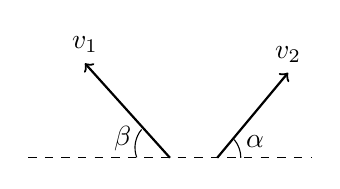
\begin{tikzpicture}[scale=0.6]

\draw[dashed] (-3,0) -- (3,0);

\draw[->,thick] (0,0) -- (-1.8,2) node[above] {$v_1$};
\draw[->,thick] (1,0) -- (2.5,1.8) node[above] {$v_2$};

\draw (-0.6,0.6) arc (-40:20:-0.6);
\node at (-1,0.4) {$\beta$};

\draw (1.5,0) arc (0:40:0.6);
\node at (1.8,0.35) {$\alpha$};

\end{tikzpicture}


\begin{enumerate}[label=\Alph*)]
\item $2\sqrt{31}$
\item $\sqrt{31}$
\item $\sqrt{244}$
\item $2\sqrt{91}$

\end{enumerate}


\item Ikki parallel yo‘ldan uzunligi $360$ m,
tezligi $54$ km/h bo‘lgan yuk poezdi va
uzunligi $140$ m, tezligi $90$ km/h bo‘lgan
passajir poezdi bir tomonga harakatlanmoqda.
Ikkinchi poezd birinchi poezdni necha sekund davomida quvib o‘tadi?

\begin{enumerate}[label=\Alph*)]
\item 50
\item 22
\item 15
\item 12.5

\end{enumerate}


\item Yuk poyezdi stansiyadan $36$ km/h tezlik bilan chiqdi.
$15$ min vaqt o‘tgach, xuddi o‘sha yo‘nalishda tezligi
$90$ km/h bo‘lgan ekspress poyezdi yo‘lga chiqdi. Yuk poyezdi yo‘lga chiqqandan keyin qancha vaqt (soat) o‘tgach va stansiyadan qanday masofada (km) ekspress poyezdi yuk poyezdiga yetib oladi?

\begin{enumerate}[label=\Alph*)]
\item 1.2; 72
\item 2; 18
\item 1; 36
\item 1/6; 15

\end{enumerate}


\item $P$ va $Q$ qishloqlar to‘g‘ri yo‘l yoqasida
bir-biridan $4000$ m masofada joylashgan. $P$ qishloqdan $Q$ tomon doimiy $8$ m/s tezlik bilan
avtomobil jo‘nadi. Shundan $30$ s o‘tgach $Q$ dan
$P$ tomon doimiy $12$ m/s tezlik bilan boshqa
avtomobil yo‘lga chiqdi.

Ular $P$ qishloqdan qanday masofada uchrashadilar (m)?

\begin{enumerate}[label=\Alph*)]
\item 1744
\item 1920
\item 2080
\item 2280

\end{enumerate}

\end{enumerate}

\begin{table}[h!]
\centering
\begin{tabular}{|c|c|c|c|c|c|c|c|c|c|}
\hline
1a & 2d & 3d & 4d & 5c & 6a & 7c & 8b & 9c & 10b \\ \hline
11d & 12a & 13a & 14a & 15c &  &  &  &  &  \\ \hline
\end{tabular}
\end{table}










\section{Notekis harakat}

\begin{enumerate}

\item Quyidagi fikrlarning qaysi biri noto‘g‘ri?

\begin{enumerate}[label=\Alph*)]
\item agar jism biror sanoq sistemaga nisbatan tinch turgan bo‘lsa, uning bu sistemaga nisbatan tezligi nolga teng bo‘ladi
\item harakatlanish vaqtini topish uchun o‘rtacha tezlikni bosib o‘tilgan yo‘lga bo‘lish kerak
\item tekis harakatda tezlikning son qiymati o‘zgarmas kattalikdir
\item harakatning o‘rtacha tezligini topish uchun bosib o‘tilgan yo‘lni harakatlanish vaqtiga bo‘lish kerak
\end{enumerate}


\item Agar jism yo‘lning $1$-yarmini $20$ s da, $2$-yarmini esa $10$ s da o‘tgan bo‘lsa,
uning o‘rtacha tezligi necha m/s? Yo‘l $240$ metrga teng.

\begin{enumerate}[label=\Alph*)]
\item 18
\item 16
\item 12
\item 8
\end{enumerate}


\item Mototsikchi $2$ soatda $90$ km yo‘l bosdi. Qolgan $3$ soatda esa
$50$ km/h tezlik bilan yurdi. Uning butun yo‘l davomidagi
o‘rtacha tezligi qanday (km/h)?

\begin{enumerate}[label=\Alph*)]
\item 35
\item 48
\item 57
\item 70
\end{enumerate}


\item Kater yo‘lning birinchi yarmini ikkinchi yarmiga nisbatan
$3$ marta katta tezlikda o‘tdi. Agar katerning o‘rtacha tezligi
$6$ km/soat bo‘lsa, uning yo‘lning birinchi yarmidagi tezligini toping
(km/soat).

\begin{enumerate}[label=\Alph*)]
\item 4
\item 8
\item 12
\item 9
\end{enumerate}


\item Agar elektropoezd yo‘lning uchdan bir qismini
$5$ m/s tezlik bilan, qolgan qismini esa
$72$ km/h tezlik bilan o‘tsa, uning o‘rtacha tezligi
necha m/s bo‘ladi?

\begin{enumerate}[label=\Alph*)]
\item 10
\item 12.5
\item 38.5
\item 18
\end{enumerate}


\item Avtomobil harakat vaqtining dastlabki $1/4$ qismini
$70$ km/h tezlikda, qolgan vaqtida $50$ km/h tezlikda
harakatlangan bo‘lsa, butun harakat vaqtidagi
o‘rtacha tezlikni toping (km/h).

\begin{enumerate}[label=\Alph*)]
\item 55
\item 63
\item 53.8
\item 60
\end{enumerate}


\item Turist yo‘lning $6$ km ini $12$ km/h tezlik bilan,
keyingi $40$ minutda esa $10$ km yurdi.
Turist harakatining boshlang‘ich bir soatidagi
o‘rtacha tezlikni toping (km/h).

\begin{enumerate}[label=\Alph*)]
\item 7.5
\item 8.5
\item 10
\item 12
\end{enumerate}


\item Qayiqning manzilga borib kelishdagi o‘rtacha tezligi
$3$ km/h va manzilga borish vaqti kelish vaqtidan
$2$ marta kichik bo‘lsa, qayiqning turg‘un suvdagi
tezligi qanday (km/h) bo‘ladi?

\begin{enumerate}[label=\Alph*)]
\item $9/8$
\item $27/8$
\item $15/4$
\item $19/4$

\end{enumerate}


\item Jism harakatining yo‘l–vaqt bog‘lanish grafigidagi $A$ nuqtadan rasmdagidek urinma o‘tkazildi va $\alpha = 60^\circ$ ekanligi aniqlandi.
Jismning $A$ nuqtaga mos keluvchi oniy tezligini toping (m/s).


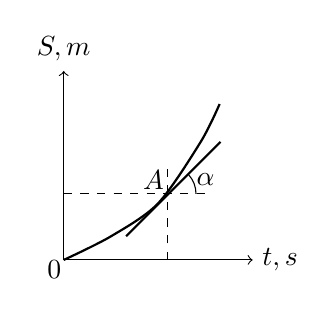
\begin{tikzpicture}[scale=0.6]

\draw[->] (0,0) -- (4,0) node[right] {$t,s$};
\draw[->] (0,0) -- (0,4) node[above] {$S,m$};

\draw[dashed] (2.2,0) -- (2.2,2);
\draw[dashed] (0,1.4) -- (3,1.4);

\draw[thick,smooth]
plot coordinates {(0,0)(1,0.5)(2,1.2)(2.9,2.5)(3.3,3.3)};

\draw[thick] (1.32,0.5) -- (3.32,2.5);

\node at (1.9,1.7) {$A$};

\draw (2.8,1.4) arc (0:42:0.6);
\node at (3,1.7) {$\alpha$};

\node at (-0.2,-0.2) {$0$};

\end{tikzpicture}

\begin{enumerate}[label=\Alph*)]
\item $1/3$
\item $\sqrt{3}$
\item 3
\item 4

\end{enumerate}


\item Quyida koordinataning vaqtga bog‘langan grafigi berilgan. $0 - t$ oraliqdagi o‘rtacha tezlik $v_1$ ga,
$t$ vaqt momentidagi oniy tezlik $v_2$ ga teng bo‘lsa,
$v_1/v_2$ nisbat nimaga teng?


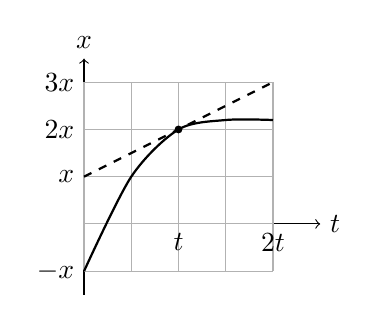
\begin{tikzpicture}[scale=0.6]

\draw[->] (0,-1.5) -- (0,3.5) node[above] {$x$};
\draw[->] (0,0) -- (5,0) node[right] {$t$};

\draw[step=1cm,gray!60] (0,-1) grid (4,3);

\node[left] at (0,1) {$x$};
\node[left] at (0,2) {$2x$};
\node[left] at (0,3) {$3x$};
\node[left] at (0,-1) {$-x$};

\node[below] at (2,0) {$t$};
\node[below] at (4,0) {$2t$};

\draw[thick,smooth]
plot coordinates {(0,-1)(1,1)(2,2)(3,2.2)(4,2.2)};

\draw[dashed,thick] (0,1) -- (4,3);

\filldraw (2,2) circle (2pt);

\end{tikzpicture}


\begin{enumerate}[label=\Alph*)]
\item 1
\item 2
\item 3
\item 4

\end{enumerate}


\end{enumerate}


\begin{table}[h!]
\centering
\begin{tabular}{|c|c|c|c|c|c|c|c|c|c|}
\hline
1b & 2d & 3b & 4c & 5d & 6a & 7d & 8b & 9b & 10c \\ \hline
\end{tabular}
\end{table}

